\documentclass[12pt]{article}

\usepackage[utf8]{inputenc}

% \usepackage[papersize={2000mm,800mm},width=2000mm,height=800mm,centering]{geometry}
\usepackage[papersize={1000mm,400mm},width=1000mm,height=400mm,centering]{geometry}

% \usepackage{mathptmx}
%\usepackage{palatino}

%\usepackage{chancery}
%\usepackage{antiqua}
%\usepackage{aboensis}
\usepackage{gfsartemisia-euler}
\usepackage[T1]{fontenc}

% \usepackage{fontspec}
% \setmainfont{QTChanceryType}

\usepackage{graphicx}
\usepackage[table]{xcolor}
\usepackage{tikz}
\usetikzlibrary{decorations.text}
\usepackage[hidelinks]{hyperref}

\pagestyle{empty}

\newcommand{\logo}{\makebox[56mm][c]{\rule{0mm}{66mm}\raisebox{12mm}{\includegraphics[width=48mm]{logo/aldc-4couleurs-3.pdf}}}}

%\pagecolor{yellow!5}

\usepackage{fontspec}


\begin{document}
%\sffamily
%\bfseries
%\color{yellow!20}
\parindent=0mm

\fontspec{QTOKCorral-Ext}
\fontsize{128pt}{128pt}
\selectfont

\unitlength=1mm
\begin{picture}(0,0)
%%%%%%%%%%%%%% FOND ET LOGOS
\put(240,-550){\includegraphics[height=600mm]{levis3.jpg}}
%\put(-5,-400){\includegraphics[height=405mm]{images/Fond-bois-tres-clair-small.jpg}}
\put(-5,-400){\includegraphics[height=405mm]{images/Fond-bois.jpg}}
\put(5,-375){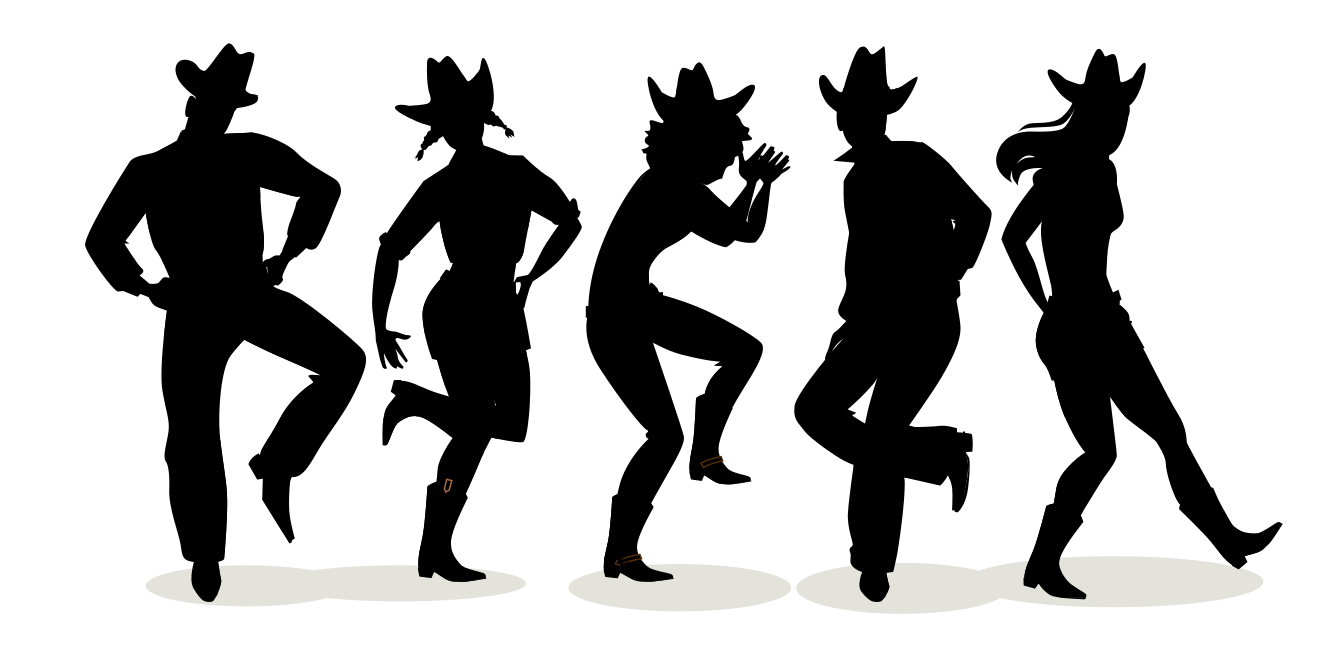
\includegraphics[width=240mm]{images/groupededanseenligne-ombre.pdf}}
\put(10,-220){\href{https://alevisdanse.github.io}{\includegraphics[height=200mm]{static/images/logo-aldc-contour-violet.pdf}}}
\put(720,-200){\href{https://alevisdanse.github.io}{\includegraphics[height=200mm]{static/images/logo-aldc-contour-noir.pdf}}}
\put(320,-260){\color{yellow!20}The Very Best of Line Dancing}
\put(318,-258){The Very Best of Line Dancing}
\put(370,-310){\color{blue!50}in the Famous High Valley of Yvette}
\put(368,-308){in the Famous High Valley of Yvette}
\put(420,-360){\color{red!50}(C'est juste un exemple de texte !)}
\put(417,-357){(C'est juste un exemple de texte !)}
\end{picture}


\end{document}


%%% Local Variables:
%%% TeX-engine: luatex
%%% End: